% Канонический TikZ-рисунок варианта 09. Править только здесь.
\long\def\figStereoV09{%
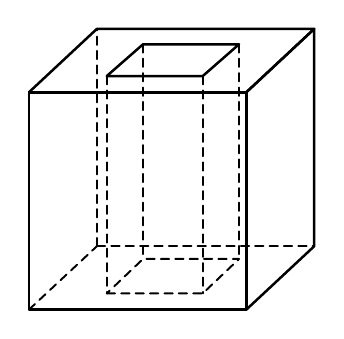
\begin{tikzpicture}[
    scale=1.15,
    line cap=round,
    line join=round,
    visible/.style={
        line width=0.9pt
    },
    hidden/.style={
        line width=0.7pt,
        dashed,
        dash pattern=on 3pt off 2.2pt
    }
]

% =================================================
% Вершины куба
% =================================================

% Передняя грань
\coordinate (A) at (0,0);
\coordinate (B) at (2.4,0);
\coordinate (C) at (2.4,2.4);
\coordinate (D) at (0,2.4);

% Задняя грань
\coordinate (A1) at (0.75,0.70);
\coordinate (B1) at (3.15,0.70);
\coordinate (C1) at (3.15,3.10);
\coordinate (D1) at (0.75,3.10);

% =================================================
% Верхнее основание вырезанной призмы
% =================================================

\coordinate (P1) at (0.86,2.58);
\coordinate (P2) at (1.92,2.58);
\coordinate (P3) at (2.32,2.93);
\coordinate (P4) at (1.26,2.93);

% Нижнее основание вырезанной призмы
\coordinate (Q1) at (0.86,0.18);
\coordinate (Q2) at (1.92,0.18);
\coordinate (Q3) at (2.32,0.56);
\coordinate (Q4) at (1.26,0.56);

% =================================================
% Скрытые рёбра куба
% =================================================

\draw[hidden] (A)--(A1);
\draw[hidden] (A1)--(B1);
\draw[hidden] (A1)--(D1);

% =================================================
% Внутренние рёбра отверстия
% =================================================

% Вертикальные рёбра вырезанной призмы
\draw[hidden] (P1)--(Q1);
\draw[hidden] (P2)--(Q2);
\draw[hidden] (P3)--(Q3);
\draw[hidden] (P4)--(Q4);

% Нижнее основание отверстия
\draw[hidden]
    (Q1)--(Q2)--(Q3)--(Q4)--cycle;

% =================================================
% Видимые рёбра куба
% =================================================

% Передняя грань
\draw[visible]
    (A)--(B)--(C)--(D)--cycle;

% Верхняя грань
\draw[visible]
    (D)--(D1)--(C1)--(C);

% Правая грань
\draw[visible]
    (C)--(C1)--(B1)--(B);

% =================================================
% Верхний край отверстия
% =================================================

\draw[visible]
    (P1)--(P2)--(P3)--(P4)--cycle;

\end{tikzpicture}
}
